\subsection{Unequal Measurement of the Two Traits}
\label{sec:unequal}

Equal block sizes and loadings make the two asymmetric ML solutions equally good. Unequal measurement resolves that equality except at particular correlations, described below, at which two different solutions fit equally well. It does not, however, force the fitted factor to become an equal composite. For equally long blocks with different loadings, the global solution always gives greater weight to the more strongly measured trait. A second, worse local minimum may still emphasize the other trait. The results below distinguish this asymmetry in the population solution from the ambiguity caused by exact exchangeability.

The reduction to two fitted loadings remains valid when block sizes and population loadings differ across blocks.

\begin{lemma}[Constant fitted loadings within blocks]
\label{lem:uniformity}
Let block A contain $m_A\ge2$ items with population loading $\lambda_A$ and block B contain $m_B\ge2$ items with loading $\lambda_B$, where $0<\lambda_A,\lambda_B<1$ and $0<\varphi<1$. Every local minimum of the one-factor ML discrepancy over free loadings and nonnegative uniquenesses has strictly positive uniquenesses. After a common sign change, its loadings are positive and constant within each block: $\alpha$ in A and $\beta$ in B. The uniquenesses are $1-\alpha^2$ and $1-\beta^2$, respectively.

\end{lemma}

Appendix~\ref{app:unequal} gives the reduction argument and the scalar equation that classifies the resulting solutions. The reduction does not require equal loadings across blocks, but it does require the population correlation structure stated in the lemma. More generally, it holds when the items are exchangeable within each block, with within-block correlations $r_A,r_B\in(0,1)$ and a positive cross-block correlation $c$ satisfying $c^2\le r_Ar_B$. This includes the common-parts and cross-loading constructions described in that appendix. Negative cross-block correlation is handled by reflecting one block. Exchangeability within blocks alone is insufficient; Appendix~\ref{app:unequal-reduction} gives a counterexample.

At zero trait correlation, the fitted factor retains the block with the larger total correlation, and
\[
F_{\min}(0)=2\min\{\TC(R_A),\TC(R_B)\}.
\]
If $\TC(R_A)>\TC(R_B)$, the minimizing covariance is $\diag(R_A,I_{m_B})$; if $\TC(R_B)>\TC(R_A)$, it is $\diag(I_{m_A},R_B)$. Equality gives these two minimizing covariances. When the two total correlations are equal but the block lengths differ, it remains open which of these solutions continues as the global solution for small positive $\varphi$. A retained two-item block has the same parameter nonuniqueness as in Theorem~\ref{thm:ml}. For equal block sizes, the larger population loading determines which block is retained.

To describe a fitted loading pattern in the coordinates of the generating traits, define covariance-matching coefficients $w_A$ and $w_B$ by
\[
l_A=\lambda_A(w_A+\varphi w_B),\qquad
l_B=\lambda_B(\varphi w_A+w_B),
\]
where $l_A$ and $l_B$ are the fitted block loadings ($\alpha$ and $\beta$ under Lemma~\ref{lem:uniformity}). The coefficients are uniquely determined for $|\varphi|<1$. We orient the fitted factor so that $w_A+w_B>0$, and we report the coefficient share $\max(w_A,w_B)/(w_A+w_B)$, which is undefined when $w_A+w_B=0$. It equals .5 for an equal composite and 1 for a single trait. We call the trait with the larger coefficient the \emph{followed trait}. This normalized coefficient share describes the fitted covariance pattern. It is not a proportion of explained variance or the trait share of an estimated factor score.

\begin{proposition}[Equal block sizes and unequal loadings]
\label{prop:unequal}
Suppose each block contains $m\ge2$ items, $0<\lambda_A<\lambda_B<1$, and $0<\varphi<1$. The global minimum is unique up to a common sign. It satisfies $\beta>\alpha$, and the trait measured by block B is the followed trait. A second local minimum, with $\alpha>\beta$ and the trait measured by block A as the followed trait, exists for some positive trait correlation if and only if
\begin{equation}
\frac{m\lambda_A^2}{1-\lambda_A^2}>(m-1)\lambda_B^2.
\label{eq:weaker-minimum-condition}
\end{equation}
When this condition holds, the second minimum exists exactly for $0<\varphi<\varphi_f$. At $\varphi_f$ it meets a saddle in a nondegenerate fold and ceases to be a local minimum. If the condition fails, including equality, the global solution is the only local minimum for every $\varphi>0$.

\end{proposition}

A fold is a correlation at which a local minimum meets a saddle point and both disappear. It is nondegenerate when this collision has the generic saddle-node form; Appendix~\ref{app:unequal-scalar} gives the conditions. Condition~\eqref{eq:weaker-minimum-condition} states that the leading eigenvalue of block A's correlation matrix after each item is scaled by its unique standard deviation, $1+m\lambda_A^2/(1-\lambda_A^2)$, exceeds the leading eigenvalue $1+(m-1)\lambda_B^2$ of the omitted block's correlation matrix. Equivalently, at $\varphi=0$ the exact fit to A alone has positive curvature in the omitted block's loading directions (Online Resource~3, Section~2.1). With four items per block and $\lambda_B=.8$, it requires $\lambda_A>.5695$. For loadings .68 and .72, the weaker-block minimum persists up to $\varphi_f=.242$; for .6 and .8, it persists only up to $\varphi_f=.017$. Thus the absence of nonglobal ML minima in Theorem~\ref{thm:ml} depends on the exchangeable design. It is not a general property of one-factor fitting to two traits.

The trait composition of a factor score differs from the coefficient share. A score $S=\bm{g}^{\top}x$ with weight vector $\bm{g}$, for the item vector $x$, has trait part $(\Lambda^{\top}\bm{g})^{\top}\theta$, where $\Lambda$ is the two-factor population loading matrix and $\theta=(\theta_1,\theta_2)^{\top}$. Its share for trait A is therefore $(\Lambda^{\top}\bm{g})_A/\{(\Lambda^{\top}\bm{g})_A+(\Lambda^{\top}\bm{g})_B\}$. For positive fitted uniquenesses, regression and Bartlett scores from the one-factor model have weights proportional to $\hat\Psi^{-1}l$ and hence the same trait share. For four items per trait, loading .7, and $\varphi=.3$, the followed-trait shares are .786 for the fitted factor, .750 for these scores, and .500 for the unit-weighted sum. In the designs examined, the score share lies between the other two; this ordering is a numerical finding, not a general theorem. When loadings differ within a block, the factor share uses block-average loadings and is an approximation.

\begin{figure}[t]
\centering
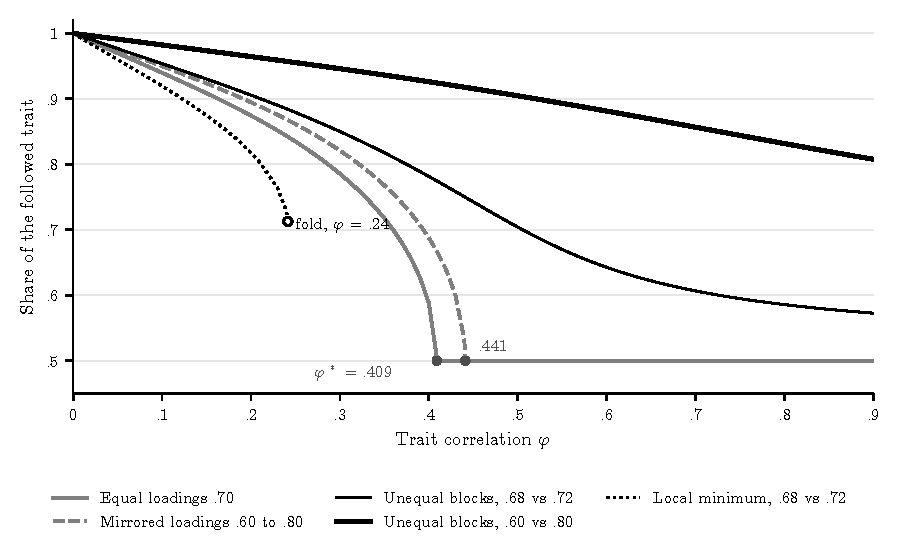
\includegraphics[width=0.85\textwidth]{fig2.pdf}
\caption{Coefficient share of the followed trait in the fitted one-factor ML model, with four items per trait. The designs have equal loadings of .70, mirrored loadings of .60, .65, .75, and .80 in each block, or different block loadings of .68 versus .72 and .60 versus .80. A share of .5 denotes an equal composite and 1 denotes one trait. For the mirrored design, the share uses block-average loadings and is approximate. The dotted curve shows the nonglobal local minimum that emphasizes the weaker block in the .68/.72 design; it ends at the fold $\varphi_f=.242$. Points on the .5 line mark where the symmetric solution loses local stability (Appendix~\ref{app:mirrored}): $\varphi^*=.409$ for equal loadings, where this is the transition, and .441 for the mirrored loadings.}
\label{fig:2}
\end{figure}

Figure~\ref{fig:2} shows that modest differences in measurement can produce substantial differences in trait representation. With loadings .68 and .72, the followed-trait share decreases smoothly from 1 at $\varphi=0$ to .77 at $\varphi=.409$, the threshold of the exchangeable design with loading .70, and to .57 at $\varphi=.9$. With loadings .6 and .8, it remains above .8 even at $\varphi=.9$. The poorer local solution can be distinguished by its discrepancy: in the .68/.72 design at $\varphi=.05$, its value is 1.25, compared with .99 at the global minimum.

Sensitivity is greatest near the exchangeable threshold. If the loadings are $\lambda-\varepsilon$ and $\lambda+\varepsilon$, Theorem~\ref{thm:cusp} in Appendix~\ref{app:unequal} shows that, for fixed interior $\lambda$ and small positive $\varepsilon$, the tilt away from equal trait representation at $\varphi^*$ is of order $\varepsilon^{1/3}$. The distance between $\varphi^*$ and the weaker solution's fold is of order $\varepsilon^{2/3}$. At $\lambda=.7$ with four items per block, a loading difference of .01 ($\varepsilon=.005$) moves the followed-trait share at $\varphi^*$ from .5 to approximately .68. The theorem concerns a local perturbation of the balanced design; its approximation is not uniform near loading zero or one.

Unequal block sizes introduce a further possibility. A longer block can dominate at low trait correlation even when its items have smaller loadings, and the favored block can change as the correlation increases. With two items loading .85 and three loading .75, the longer block is favored initially, whereas the shorter block is favored above $\varphi=.758$. Near $\varphi=1$, the comparison depends on $m_k(m_k-1)\{\lambda_k^2/(1-\lambda_k^2)\}^2$ for blocks $k=A,B$. For $.5\le\varphi<1$, these statements follow from the proof in Online Resource~3, Section~2.6. For $0<\varphi<.5$, where a worse local minimum favoring the shorter block can coexist, a computer-assisted interval-arithmetic certificate reported there (\texttt{checks/unequal\_example\_certificate.py}) shows that the minimum favoring the longer block is the unique global solution.

Such a change need not be continuous. With unequal block lengths, two local minima favoring different traits can coexist and exchange global status. At the exchange correlation they fit equally well, and the global solution jumps between them. For two items loading .90 and four loading .70, this occurs at $\varphi\approx.326$, where the share of the coefficient sum $w_A+w_B$ belonging to the shorter block's trait jumps from .10 to .92 (Online Resource~3, Section~2.6). In the example above the change is instead a smooth crossing on a unique global branch. Appendix~\ref{app:unequal} gives the exact scalar comparison and additional results for mirrored heterogeneous loadings. These extensions preserve the main implication: good approximation by one factor does not determine how that factor represents the two traits.
